\chapter{船岸连接系统结构与分析}

船岸连接(Ship-to-Shore Connection),在不同的文献中有不同的名称,如冷熨烫(Cold Ironing)、岸侧电源(Shore-Side Electricity,SSE)、
岸电供电(Onshore Power Supply,OPS)、船舶岸电系统(Alternative Maritime Power Supplly,AMPS)。
虽然名称有所不同,但它们都涉及到停泊船舶靠港后关闭其船载辅助发动机,并使用港口提供的清洁能源为船载主要系统供电,
满足所有如照明、制冷和货物卸设施等船载设备的电力需求。这种技术允许停泊的船只使用船舶岸电,而不是依靠辅助发动机产生的
电力,从而减少港口污染物的排放。

\section{船岸连接系统的组成}

如图\ref{fig:船岸连接系统示意图}所示,船岸连接系统是由三个基本部分组成:岸侧电力系统和基础设施、电缆管理系统和船侧连接系统。

\begin{figure}[!htp]
	\centering
	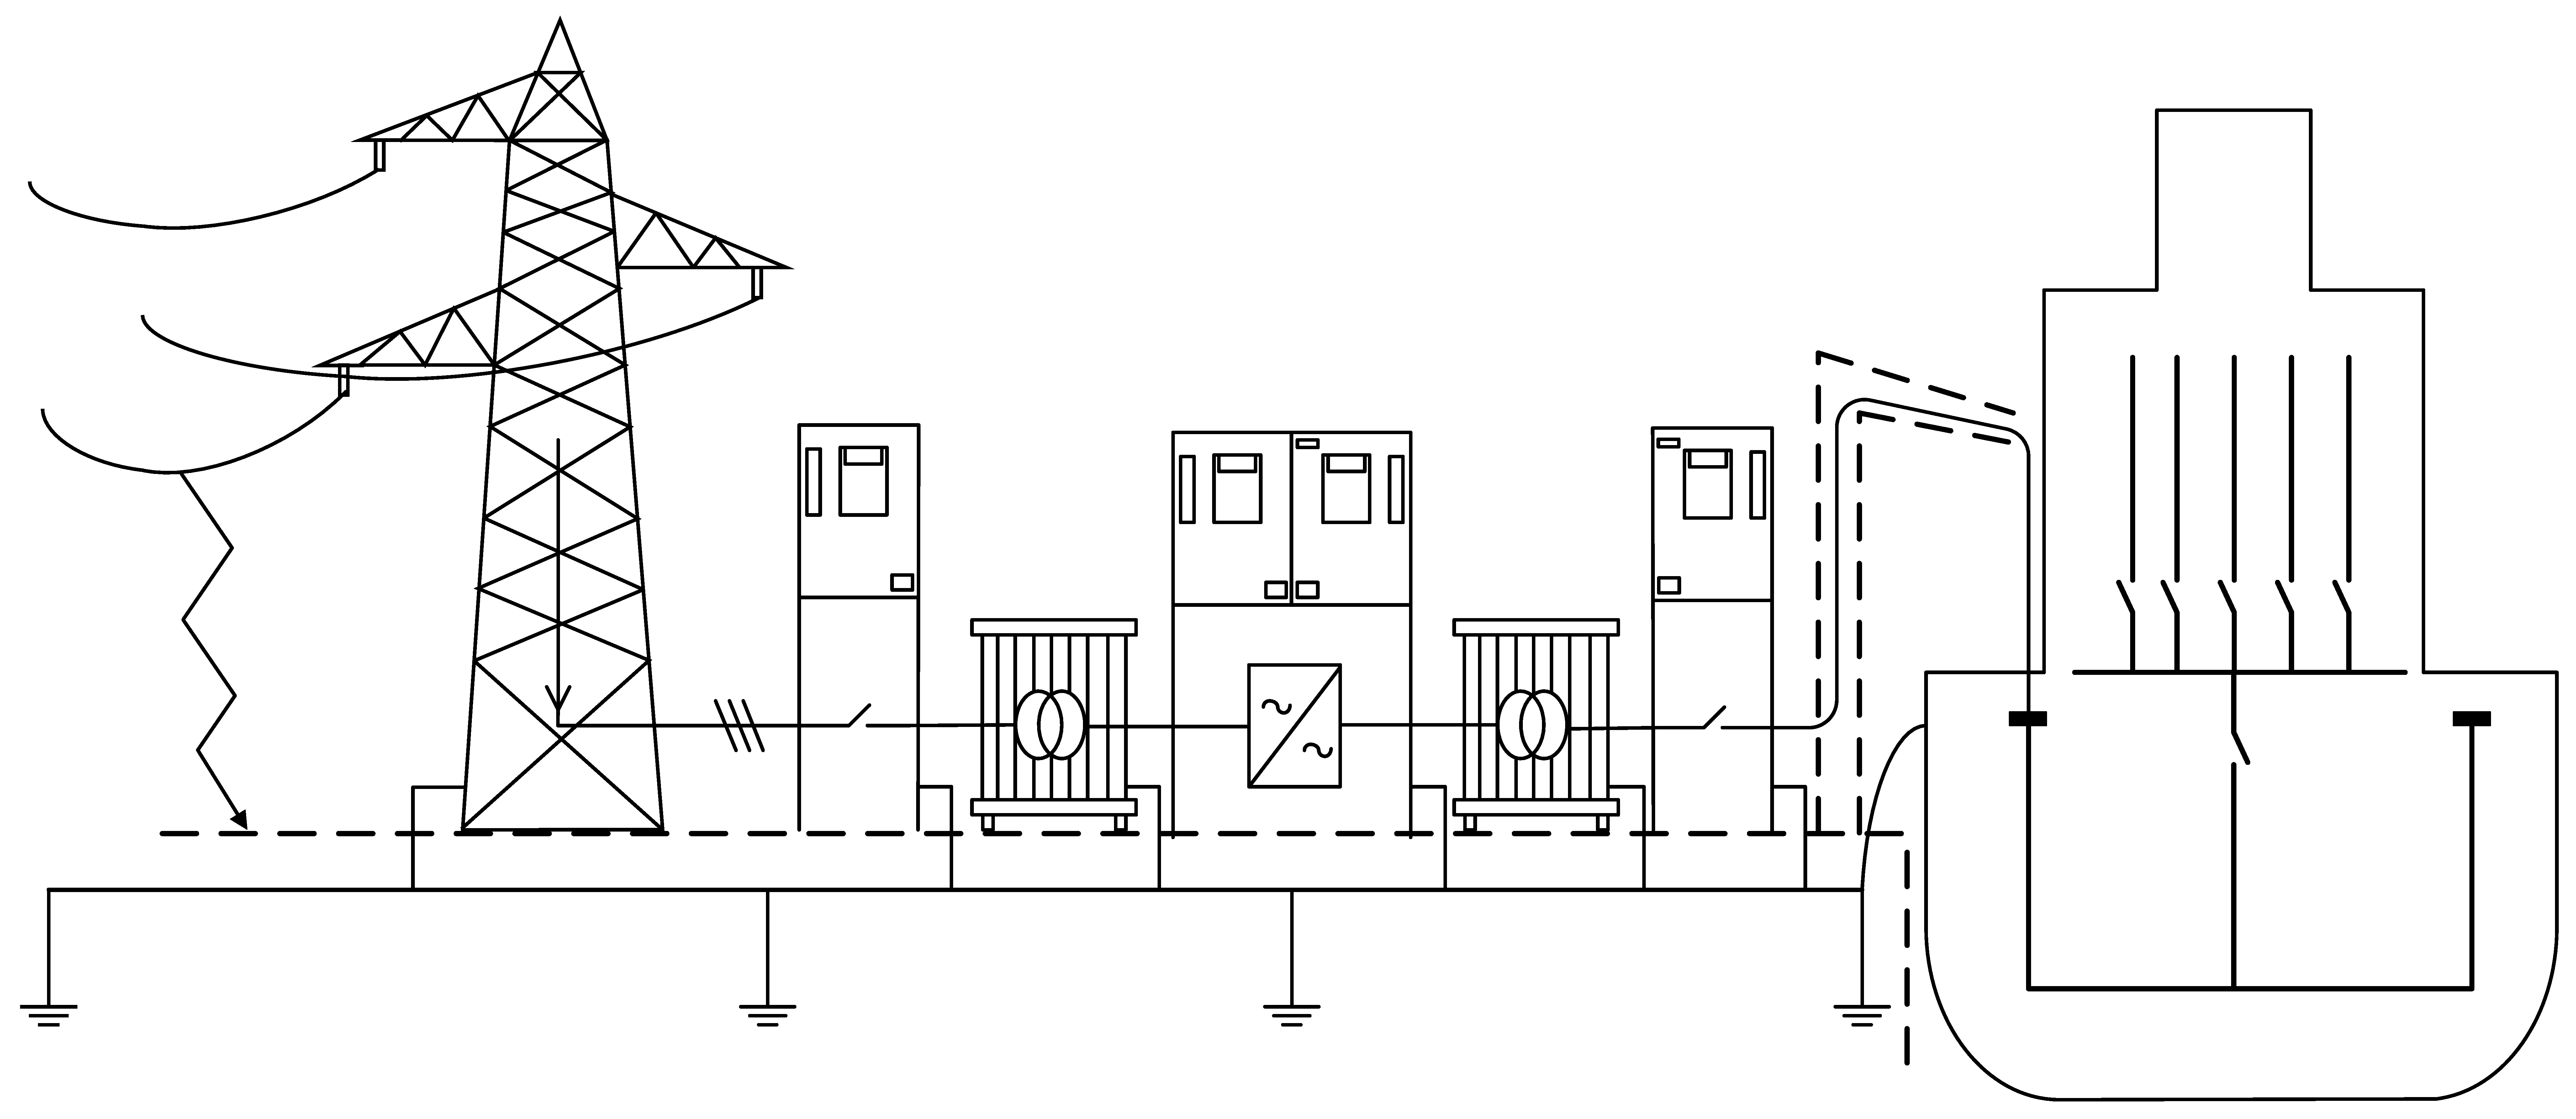
\includegraphics[width=0.95\textwidth]{chapter2/船岸连接系统示意图.pdf}
	\caption{船岸连接系统示意图}
	\label{fig:船岸连接系统示意图}
\end{figure}

岸侧电力系统负责将高压变电站的电力传输到泊位附近的连接点,即终端配电箱,以不间断的方式在船舶电力接收系统之间切换等。首先通过变压器将电网高压转换为低压。
随后,变流系统将对网侧电压变压变频,并通过变压器升至船舶电力系统所需的电压。船岸连接系统应用的电压等级不同,
所需电压由船舶类型决定:一般远洋货轮,大型集装箱船采用高压岸电,小型散货船主要采用低压。其中,岸电系统的核心部分是岸侧变流系统。
国外一些国家的电网(美国、加拿大等),一些客船的电力系统的电网频率通常为60Hz。
在电网频率为60Hz的国家中,船岸连接系统实现变得相对容易,然而在电网频率为50Hz的中国,欧洲诸国与一些其它国家,
为岸侧部分提供额外的变频装置是岸电系统所必需的。交流电实现50Hz到60Hz的转变通常有两种解决方案:静态变换器或旋转变换器(如\ref{fig:传统旋转变频与静态电源变频对比}所示)。
考虑到码头的现代全电动邮轮通常需要8–12\si{MW}\cite{SP15},在大容量的船岸连接系统中,岸电变流系统需要满足这种功率需求。
同时,可以承受足够的短路电流,使安装在船舶上的继电保护系统能够正常发挥作用。

\begin{figure}[!htp]
	\centering
	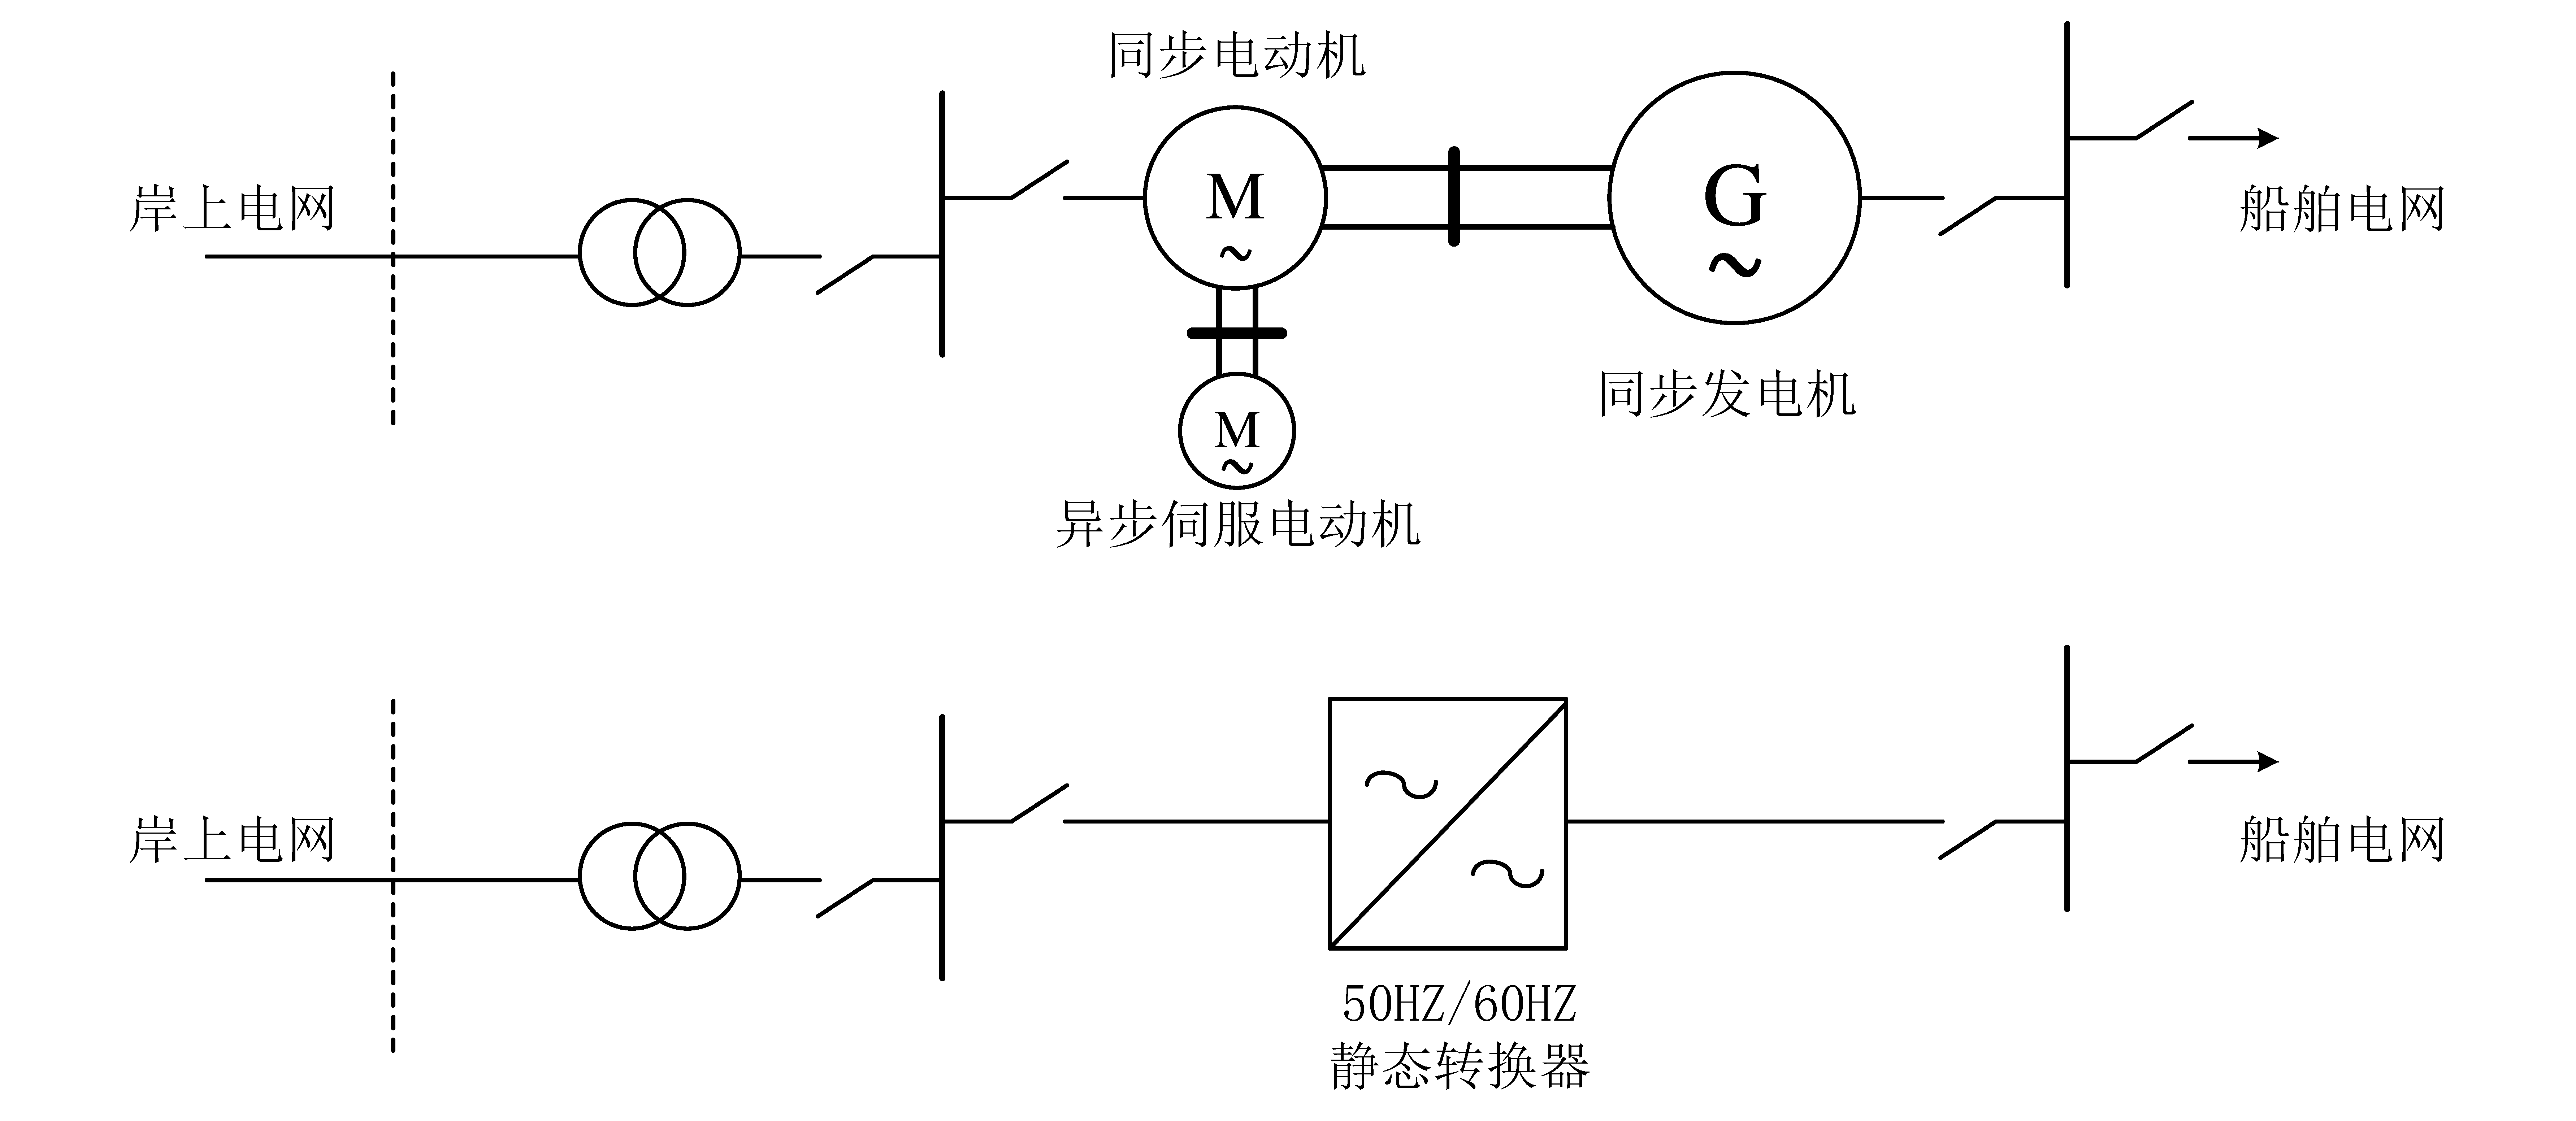
\includegraphics[width=0.85\textwidth]{chapter2/旋转形态转换器对比.pdf}
	\caption{传统旋转变频与静态电源变频对比}
	\label{fig:传统旋转变频与静态电源变频对比}
\end{figure}

电缆管理系统包括连接岸侧连接点、船载受电设备的电缆和设备。电缆连接设备必须满足电缆的收放功能,与快速连接的能力,
不使用时应存放在船上、岸上或者驳船上。船侧连接系统(图\ref{fig:船侧连接系统})是在原有的电力系统上增加接受单元,包括电缆绞车、变压器以及相关控制系统等。

\begin{figure}[!htp]
	\centering
	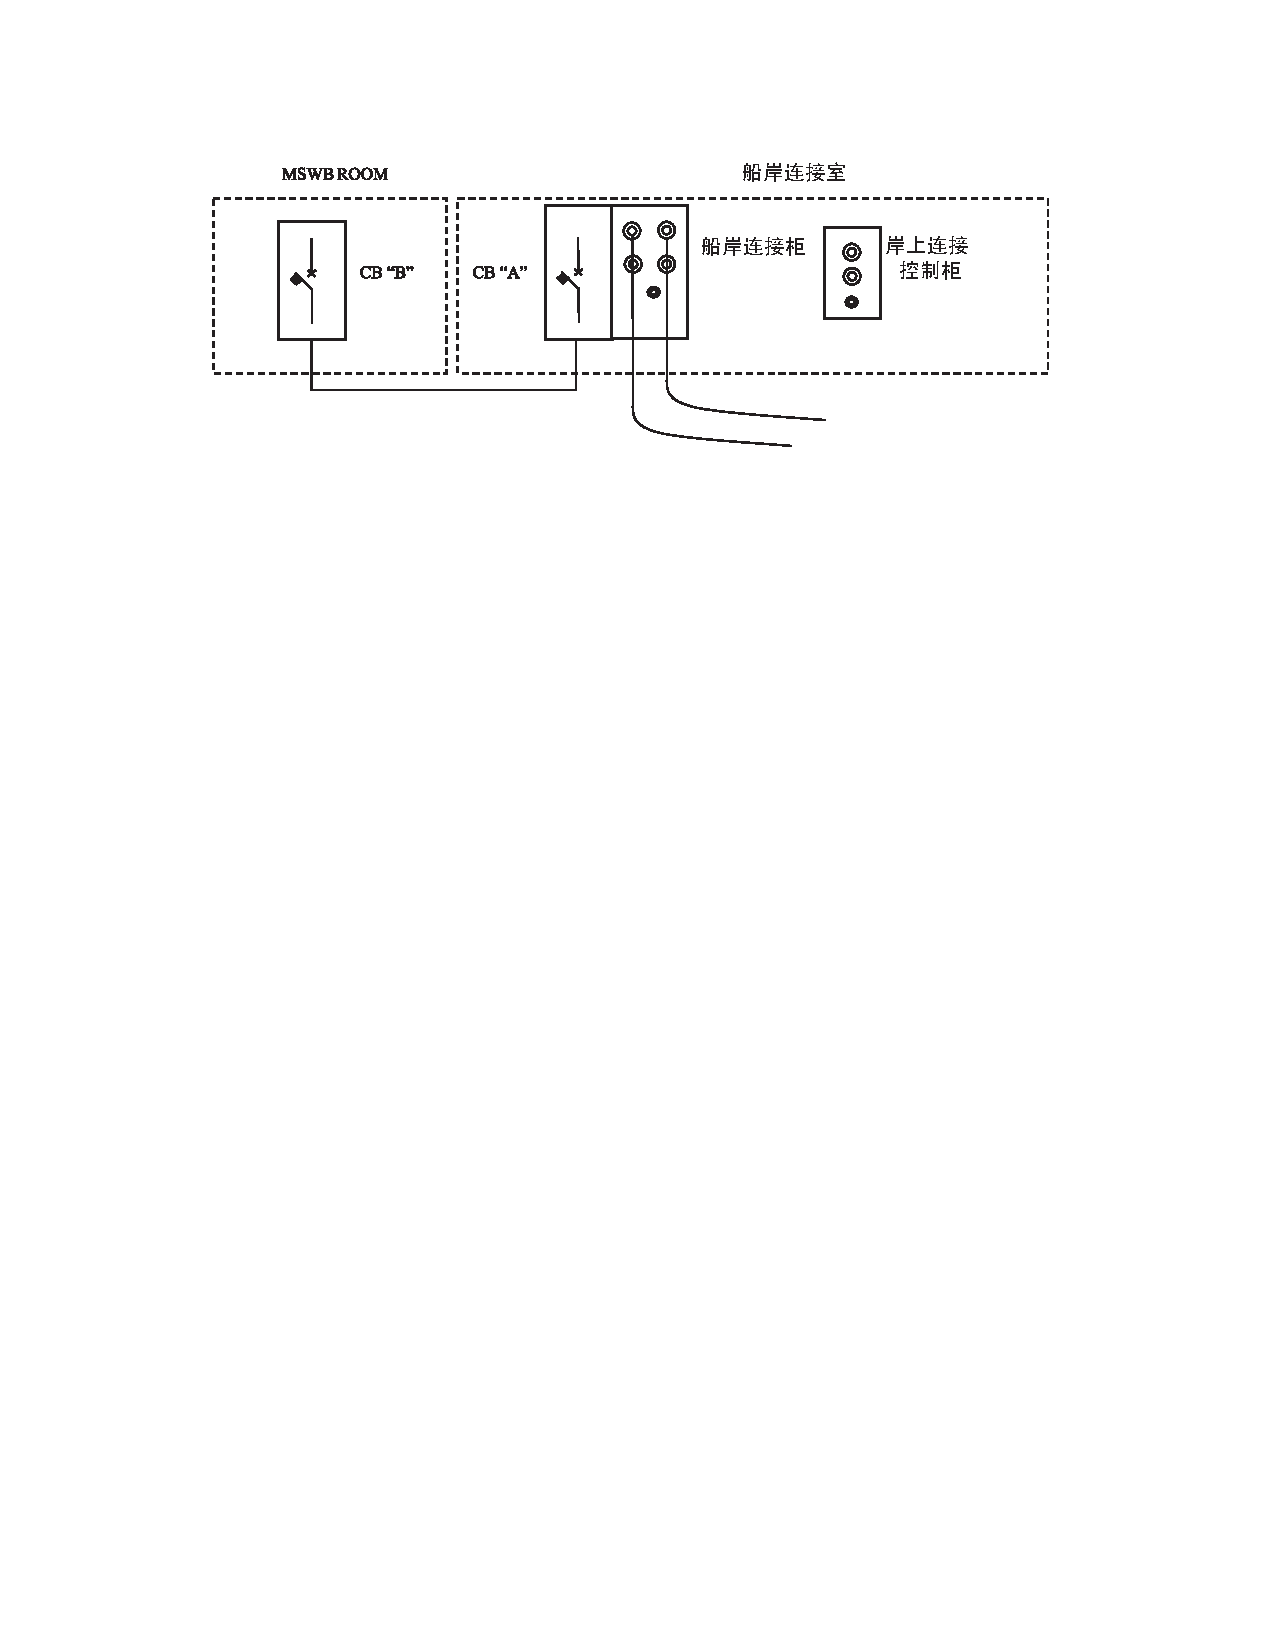
\includegraphics[width=0.85\textwidth]{chapter2/船侧船岸连接部分.pdf}
	\caption{船侧连接系统\cite{SP15}}
	\label{fig:船侧连接系统}
\end{figure}

\section{船岸连接系统的分类}

根据船舶电网的电压等级可以将船舶分为,低压船舶,和中压船舶。一般,将电压等级440V\~{}690V的船舶

目前我们对于船舶的划分是根据其船上的电力系统的电压等级,通常分为低压船舶和中压船舶。将电压为440V/690V船舶
划分为低压船舶,中压船舶则是使用6.6KV/11KV的电压。而在岸电电源中,则将6.6KV/11KV的电压上船归类为高压上船
方式。通常低压岸电电源只能给低压440V/690V船舶供电;然而高压岸电电源不仅可以直接给中压6.6KV/11KV的船舶供电,
而且还能够经过二次变换给低压440V/690V的船舶进行供电。国外先进港口近年新建设的船舶供岸电电源大都采用了高压岸
电电源,例如洛杉矶港、西雅图港、哥德堡港、西雅图港等。目前船舶方面的国际标准IEC 60092-510中就很明确的指出
岸电电源采用的上船电压等级是6.6KV/11KV,因此高压岸电则是未来我国港口岸电电源发展的主要方向。 
船载电站的发电机按电压等级可分为
高压和低压。高压船载电站的电压等级包括11 kV、6.6kV(60Hz)和6kV(50Hz),低压船载电站的电压等级包括400V(50Hz)
和440伏(60赫兹)。

国内港口可分为海港、江港、内河港(河、湖),停靠的船舶种类各异。一般外轮大多停泊于海港和部分江港,外轮使用的
电压频率一般为60Hz,电压等级为高压6.6kV、低压440V,与我国电网电制不统一,不可直接供电,必须通过变压变频之后
方可向船舶供电。国内船舶使用的电压频率和电压等级一般与电网一致,可直接供电。港口建设船舶岸基供电系统应充分考
虑港口情况、码头泊位类型、船舶电制和船舶辅靠港负荷容量等,并依此来选择合适的岸电产品。根据不同船舶用电需求,
本文将港口岸电系统按照应用需求分为“高压岸电、低压岸电及小容量岸电”等3类岸电应用形式。

\subsection{高压岸电供电系统}

高压岸电供电系统(如图\ref{fig:高压岸电供电系统}所示)用于沿海大型港口码头,可为靠港用电容量超过800kVA的船舶
提供电源\cite{SP16}。

高压上船模式是将码头电网10kV(6kV)/50Hz高压电源通过变压变频装置转换为6.6(/6)kV 、60Hz/50Hz高压电源,接入
船载电源系统供船上设备使用,变压变频装置放置在码头配电房内,在码头处配置高压岸电接电箱。高压上船可以减少电缆
根数(一般只需1根或2根电缆),但对于大多数船舶来说,使用高压岸电需要进行改造。

\begin{figure}[!htp]
	\centering
	\includegraphics[width=0.95\textwidth]{chapter2/高压岸电系统.pdf}
	\caption{高压岸电供电系统}
	\label{fig:高压岸电供电系统}
\end{figure}

\subsection{低压岸电供电系统}

低压岸电系统一般用于沿江、内河小型港口码头,可为靠港用电容量低于800kVA的船舶提供电源。当船舶靠港用电容量超过
400kVA时,如使用低压岸电系统,一般需接驳数根低压电缆,接驳时间长,难度大,因此建议靠港用电容量超过400kVA的
船舶使用高压岸电上船方式。

低压上船模式是将码头电网10kV、50Hz高压电源变频、变压转换为450(/400)V、60Hz/50Hz低压电源(双频供电),直接
接入船上受电设备使用。如果码头泊位只停靠50Hz的船舶,不需安装变频装置,直接使用380V/50Hz市电供电,变压变频
装置放置在码头配电房内,在码头设置低压岸电接电箱。使用低压岸电的船舶一般不需改造,只需要为穿用电缆配置相应
的电缆接头即可使用。

\begin{figure}[!htp]
	\centering
	\includegraphics[width=0.95\textwidth]{chapter2/低压岸电系统.pdf}
	\caption{低压岸电供电系统}
	\label{fig:低压岸电供电系统}
\end{figure}

\subsection{小容量岸电供电系统}

小容量岸电设施主要安装于停泊散货船一类的小型港口码头,针对内河、湖停靠的1000t级以内的小型船舶进行供电,船舶
电制为380V/50Hz,船舶用电主要满足船舶生活照明用电,容量一般小于20kVA。

将码头电网10kV、50Hz高压电源经变压器转换为380V三相低压电源,在码头建设小容量岸电接电桩,接入船上供受电设备
使用。

\begin{figure}[!htp]
	\centering
	\includegraphics[width=0.95\textwidth]{chapter2/小容量岸电系统.pdf}
	\caption{小容量岸电供电系统}
	\label{fig:小容量岸电供电系统}
\end{figure}

\section{船岸连接系统供电模式及对比}

(1)低压岸电/低压船舶

这种供电模式具体是指由低压岸电电源向低压船舶供电。最典型的应用案例是美国洛杉矶港的直接供电方式,其过程为:
港口的高压电先经码头的变电站降至6.6KV并通过地下电缆连接至码头岸电箱。为了节约港口空间,将6.6KV到
440V的降压变电箱装置在码头和船舶之间可以移动的驳船上,经由移动驳船上的电缆和岸电相连。
我国的上海外高桥二期采用的也是这种供电模式,只不过中间加有变频环节。该供电模式的优点是使用很灵活,不
需要对码头进行改造。缺点是需要多根电缆进行供电,连接较为不方便。

(2)高压岸电/高压船舶

这种供电模式具体是指由高压岸电电源向高压船舶供电。最典型的案例是美国长滩港的60Hz直接供电方式。与低压
岸电/低压船舶供电模式相比,高压岸电/高压船舶供电模式没有中间的降压环节,可以由码头岸电箱向高压船舶直接供电。
此方案的优点是高压上船,只需要一根电缆即可,因此安装便利,连接快捷,节省了操作时间。缺点是当给低压船舶供电时,
需要给受电船舶或者岸边安装降压变压器。由于没有变频环节,因此不能给频率为50Hz的船舶供电。

(3)高压岸电/低压船舶

这种供电模式具体是指由高压岸电电源向低压船舶供电。最典型的案例是瑞典哥德堡港
50Hz直供电方式,其过程为首先将电网高压经由变电站降至6\~{}20KV并电缆接至码头岸电箱,然后由一根高压
电缆连接上受电船舶,最后经由船载变压器降压至受电船舶所需的电压等级即可。我国的连云港也是采用的这套方案,只
是中间加入了变频环节。该方案的优点也是只需一根高压电缆上船即可,连接方便,安装快捷。缺点是需要在岸边或船上
安装固定变压器,即对码头或船舶进行一定改造,成本比较高。由于没有变频器,同样无法为电制为60Hz的船舶供电,
限制了适用范围。

\begin{table}[!htp]
	\centering
	\caption[船用岸电供电方式比较]{船用岸电供电方式比较}
	\label{tab:船用岸电供电方式比较}
	\resizebox{\textwidth}{!}{%
	\begin{tabular}{c}
		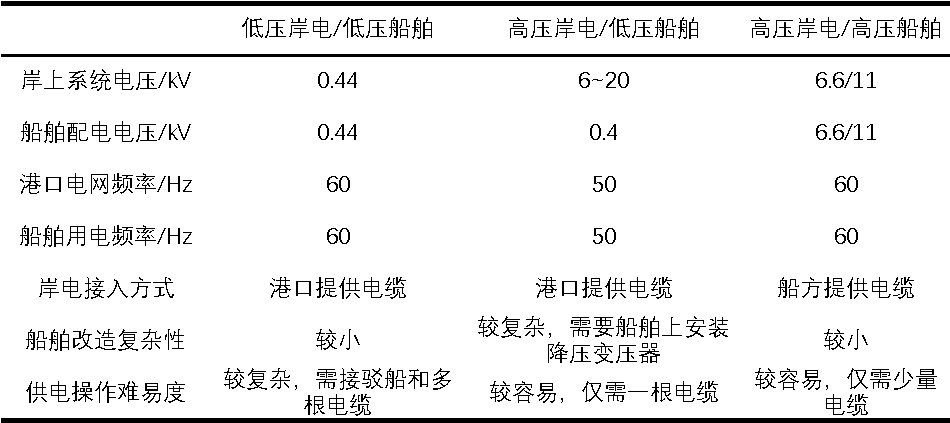
\includegraphics{chapter2/船用岸电供电方式比较.pdf} 
	\end{tabular}
	}
\end{table}


\section{船岸连接系统分布形式}

\subsection{分布式配置形式}

配置形式如图\ref{fig:分布式岸电结构}所示,港口的变电站中只安装一个大容量的变压器作为主变电站,它的原边与岸上的电网直接连接,码头上的每个泊位都安装一个
小容量的分变电站,在每个拍位的分变电站中都分别安装两个变压器和一个变流器,其中一个变压器将来自港口主变电站的
电压降为变流器所需要的电压,另外一套变压器将变流后的电压调整到靠港船舶所需要的电压。陆上电力网经过主变电站后,
电压一般降为34.5KV,然后通过地下电缆将电力传输到码头上每个泊位的分变电站中,泊位分变电站中的变流器能够将50Hz
的交流电转换为60Hz,变压器能够将电压调整到需要的等级,按照靠港船舶的需要提供不同电压、不同频率的电能。这种方
式的配置形式比较稳定可靠,具有很强的容错能力,某个泊位分变电站出现故障对其它泊位都不会产生影响。但是送种方案
也有很大的缺点,每个泊位都要安装分变电站,大大占用了本来就很不宽敞的码头空间,同时每个分变电站都要配备两套变
压器和一套变流器,所以投资也较大。

\begin{figure}[!htp]
	\centering
	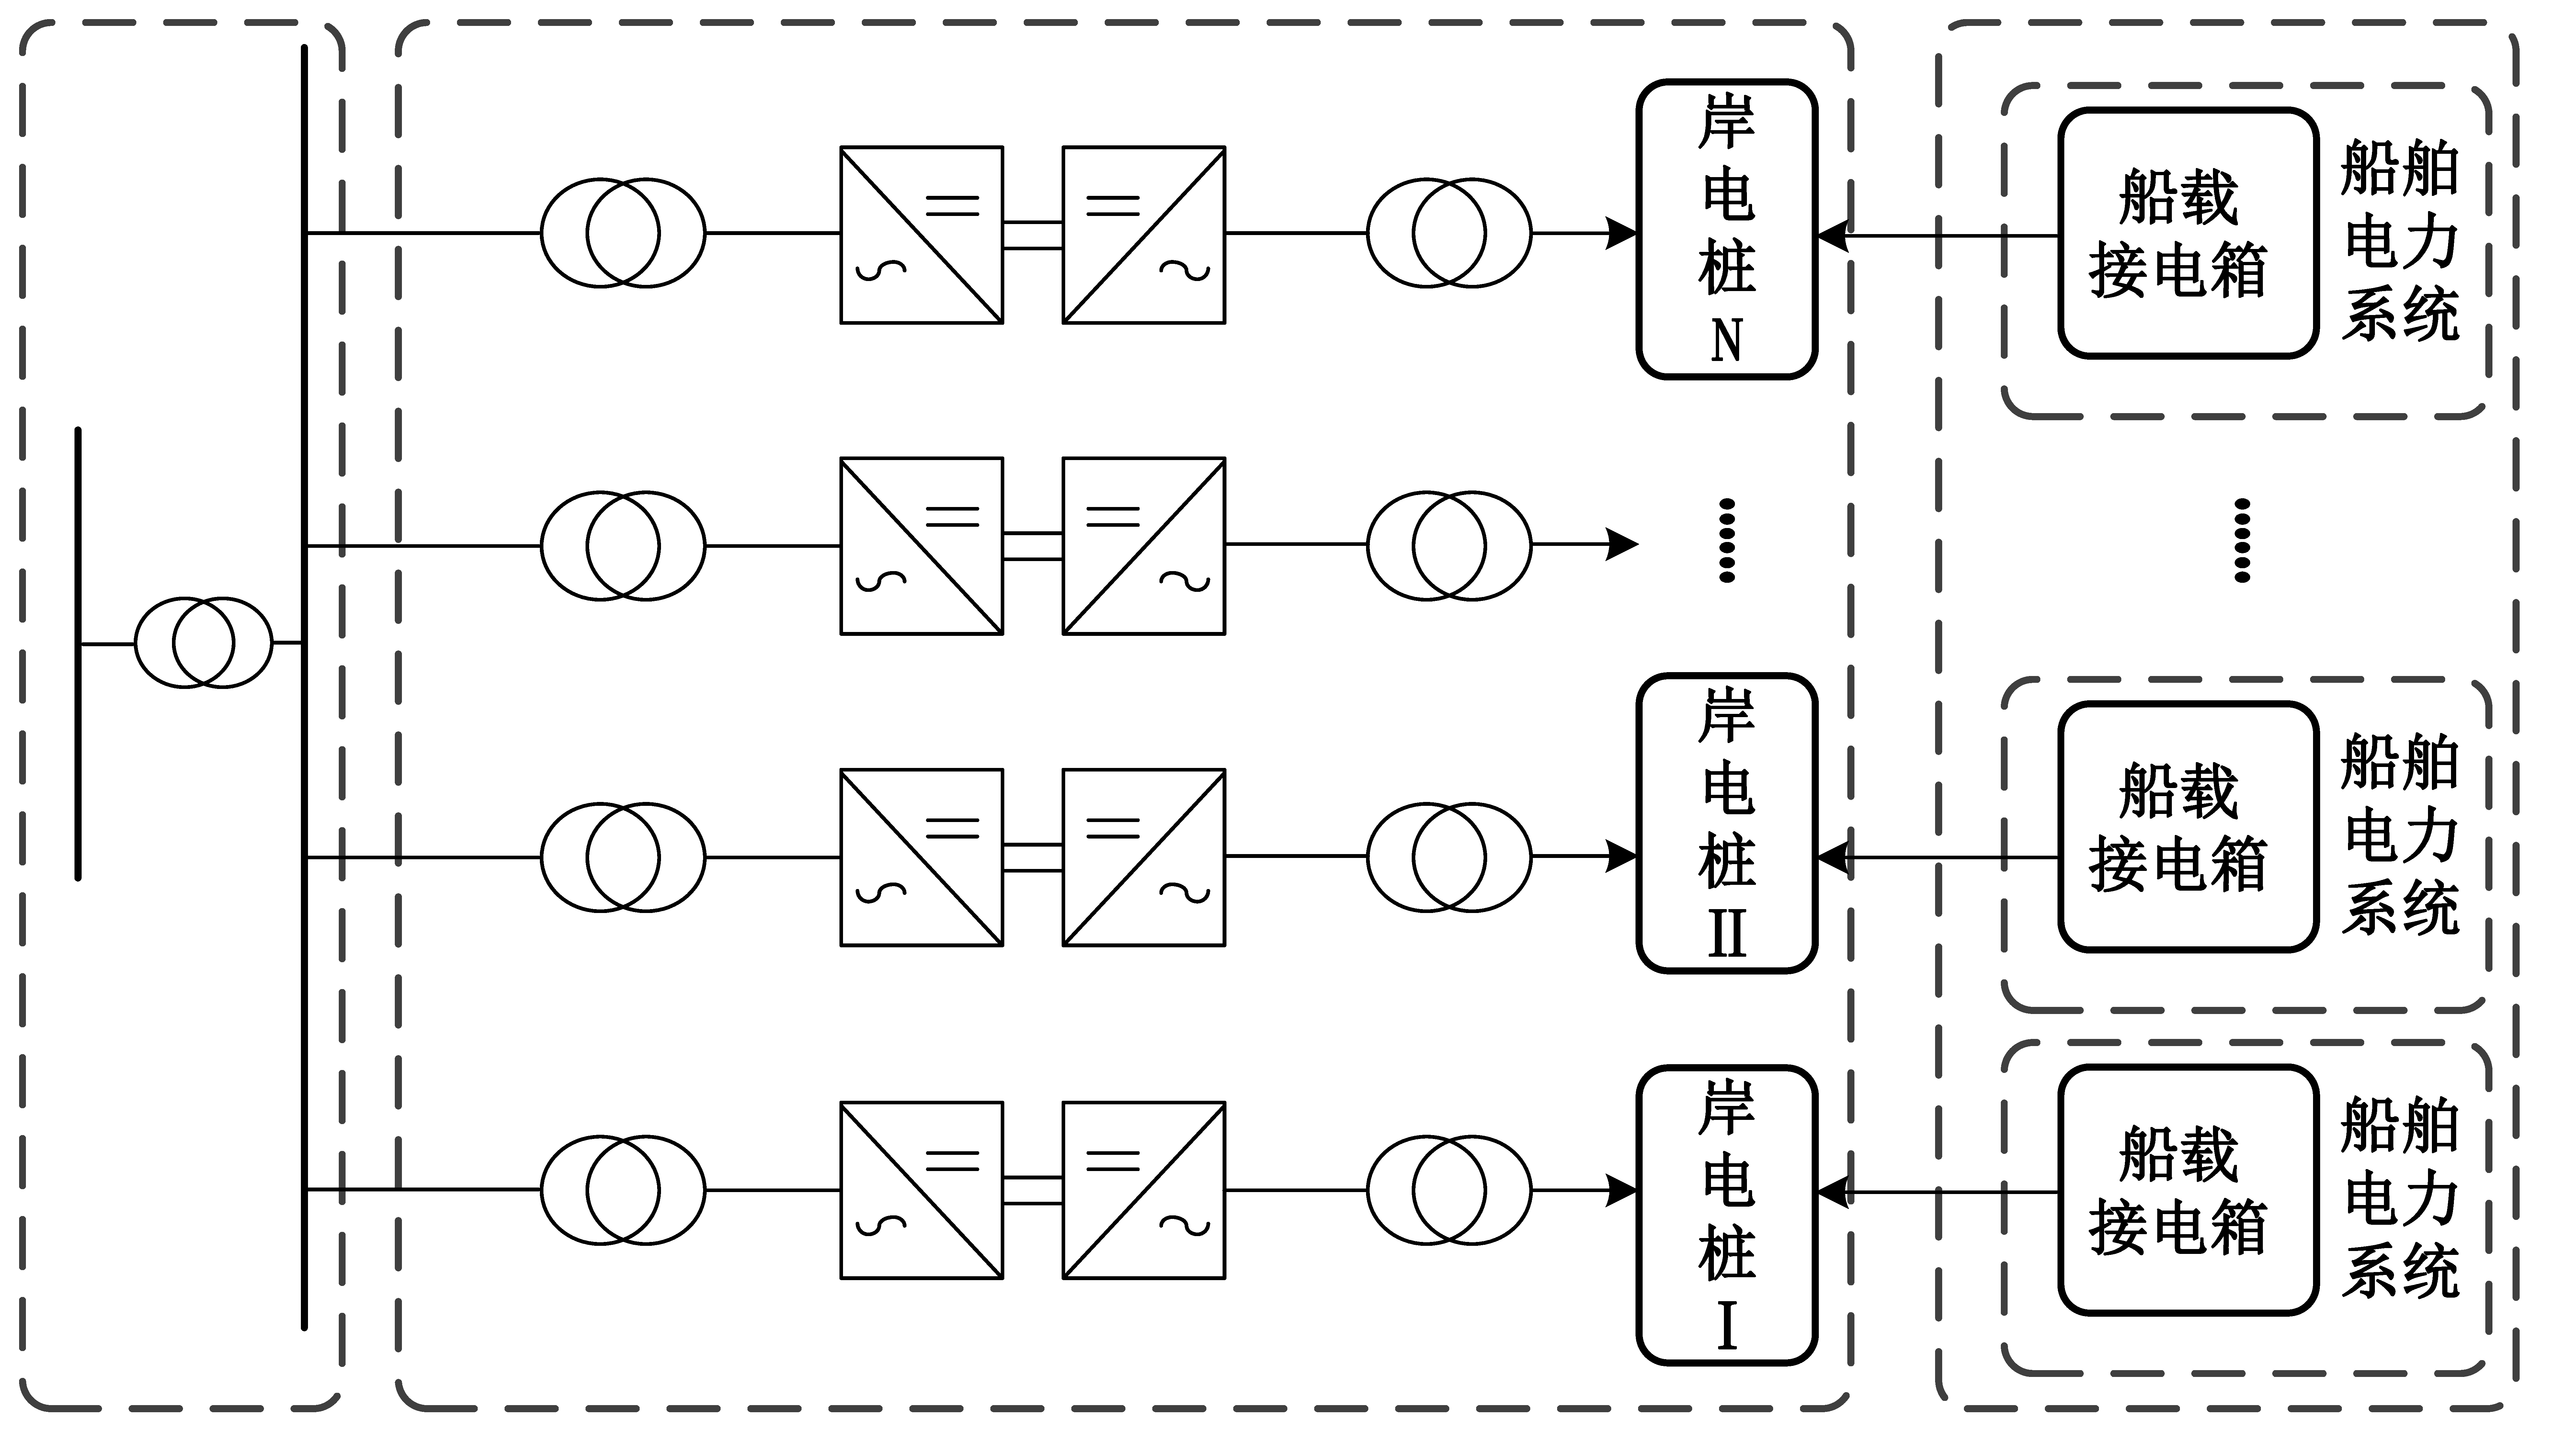
\includegraphics[width=0.9\textwidth]{chapter2/分布式岸电电源.pdf}
	\caption{分布式岸电结构}
	\label{fig:分布式岸电结构}
\end{figure}

\subsection{集中式配置形式}

配置形式如图\ref{fig:集中式岸电结构}所示,在送种配置形式中,只在港口的主变电站中安装变频设备,而在泊位上的分变电站只需配备变压设备。陆上电力网电能通过
主变电站后,既能提供60Hz的电压(通过主变电站的变流设备进行变频),也能提供50Hz的电压(不通过变频设备)。每个泊位
都有两个接电桩,分别提供60Hz和50Hz的电能,变压器能够将电压进行调整到合适的等级,靠泊船舶根据自身需要选择不同
频率的接电粧。这种配置形式的特点是将变流设备统一整合到港口的主变电站中,大大降低了占地空间,对泊位的改造要求不
高,节省了很大的初投资。但是其缺点也较明显,因为整个港口只有一套变流设备,所容错能为较差,一旦这套变流设备出现
故障,将会影响到整个港口所有泊位的岸电供应能力。但是均衡利与弊,这种配置形式的岸电电源是现在整个船舶岸电市场的
发展方向。

\begin{figure}[!htp]
	\centering
	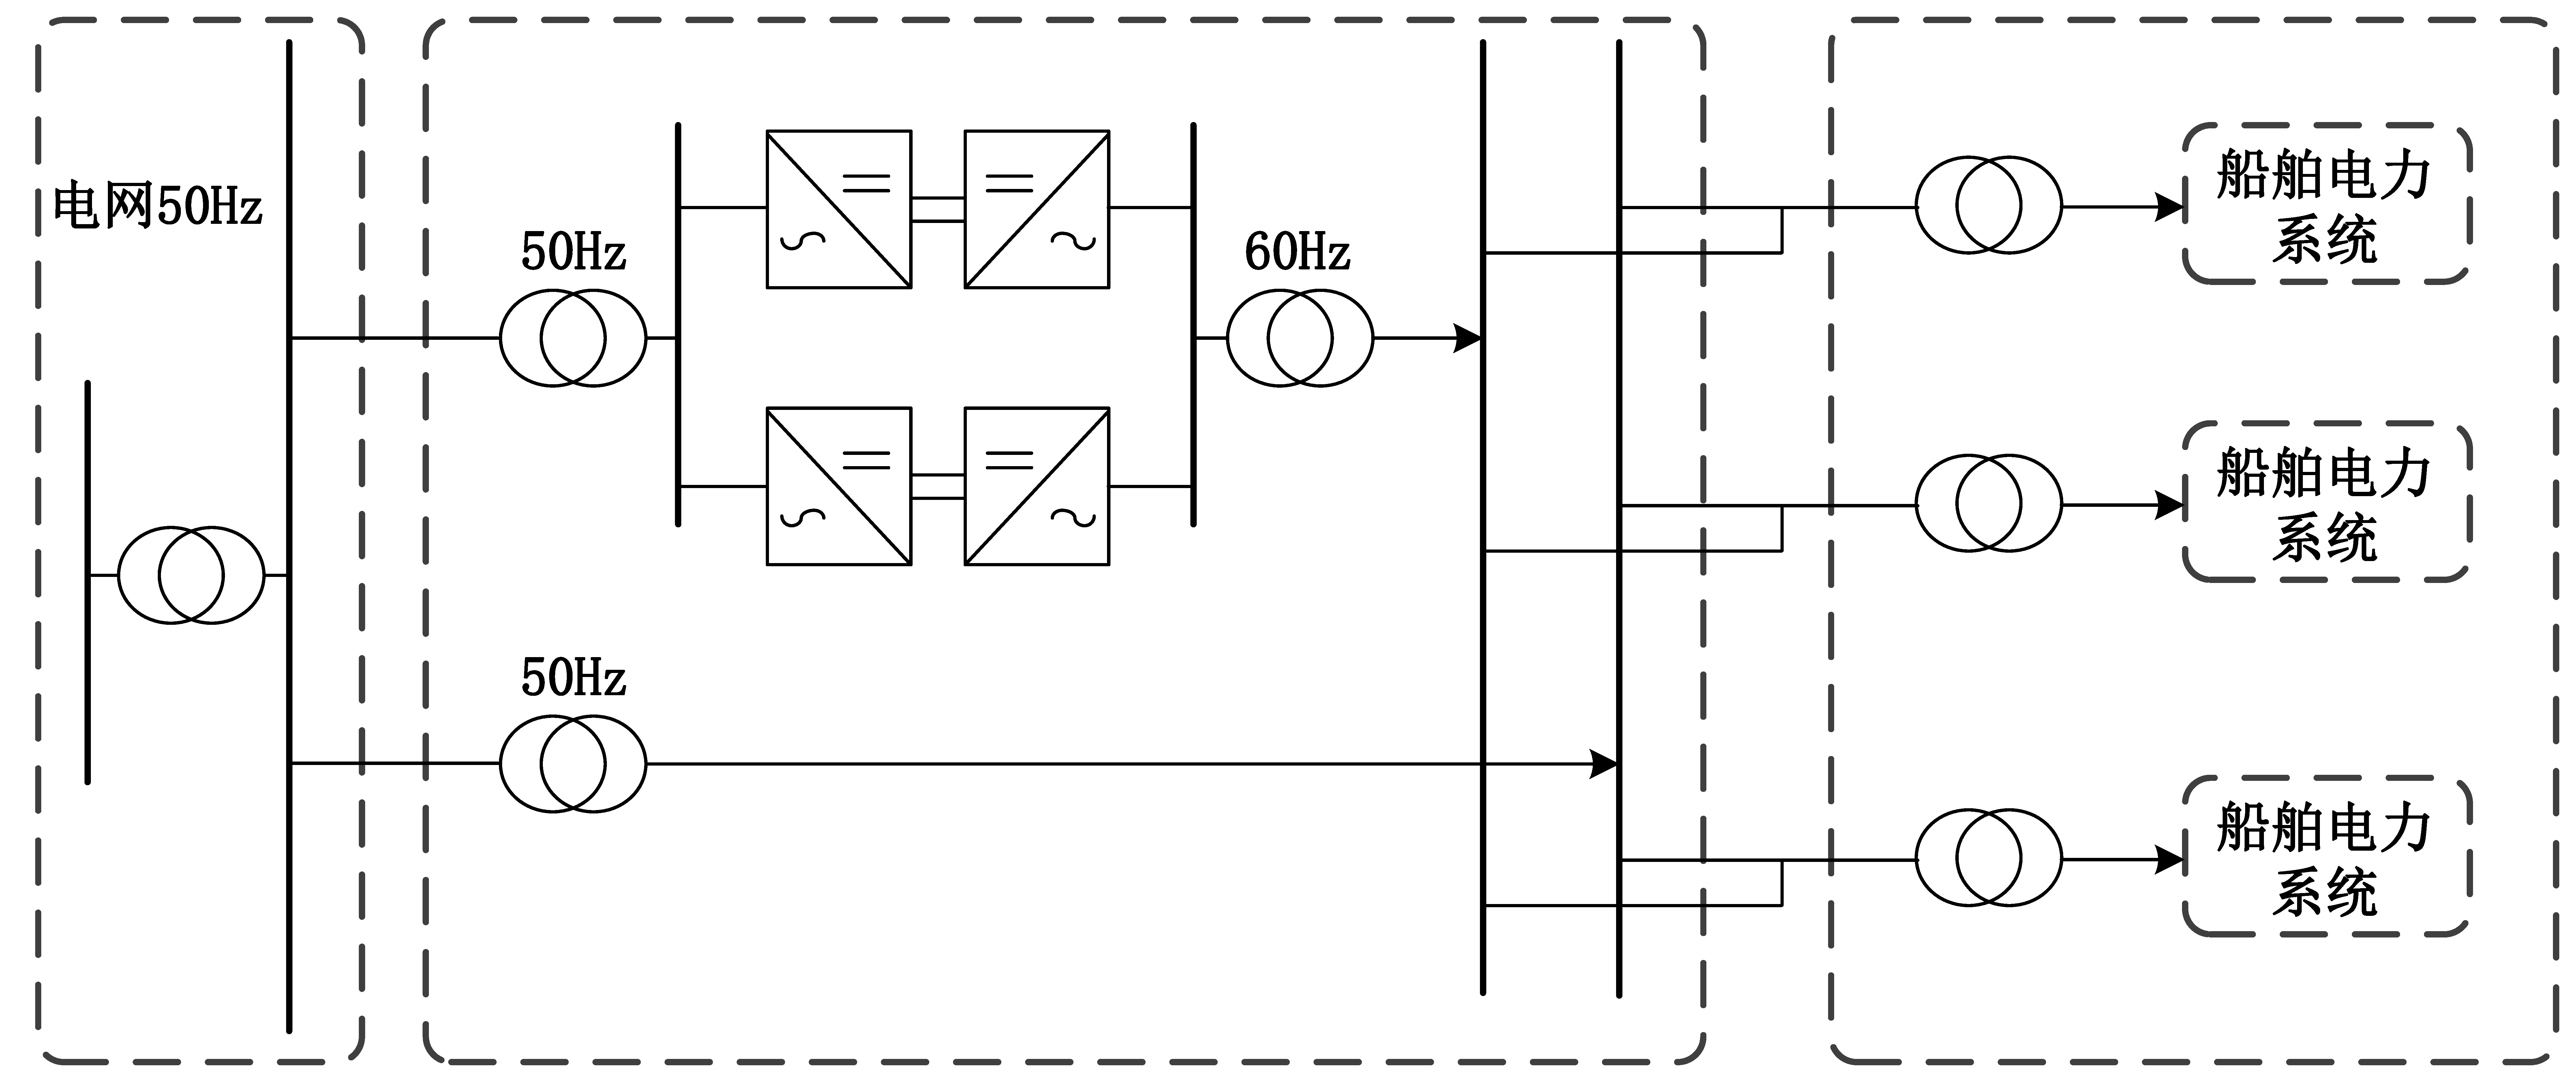
\includegraphics[width=0.9\textwidth]{chapter2/集中式岸电电源.pdf}
	\caption{集中式岸电结构}
	\label{fig:集中式岸电结构}
\end{figure}

\subsection{直流输电式形式}

配置形式如图\ref{fig:直流输电岸电结构}所示,按照这种配置形式的要求,变流设备被分成两个部分(整流部分和逆变部分),整流设备安装在港口主变电站中,逆
变部分安装在泊位上。港口主变电站的降压变压器将陆上电力网的电压降低后,连接到整流设备上,交流电经过整流设备的整
流后变换为直流电,然后电能通过电缆直流的形式传输到泊位岸边。泊位上的分变电站中配置逆变器,变频器将直流电逆变为
60HZ的三相交流电,最后 通过变压设备调整后连接到靠港船舶电网上。这种配置形式优点是直流传输损耗较低,能够节省资源,
但是由于每个泊位上都必须安装一套逆变器和一套变压器,所以对泊位空间的占用也较为严重,况且依照当前的工程水平,直流
输电技术成本较高,总之这种配置形式的岸电电源使用较少。

\begin{figure}[!htp]
	\centering
	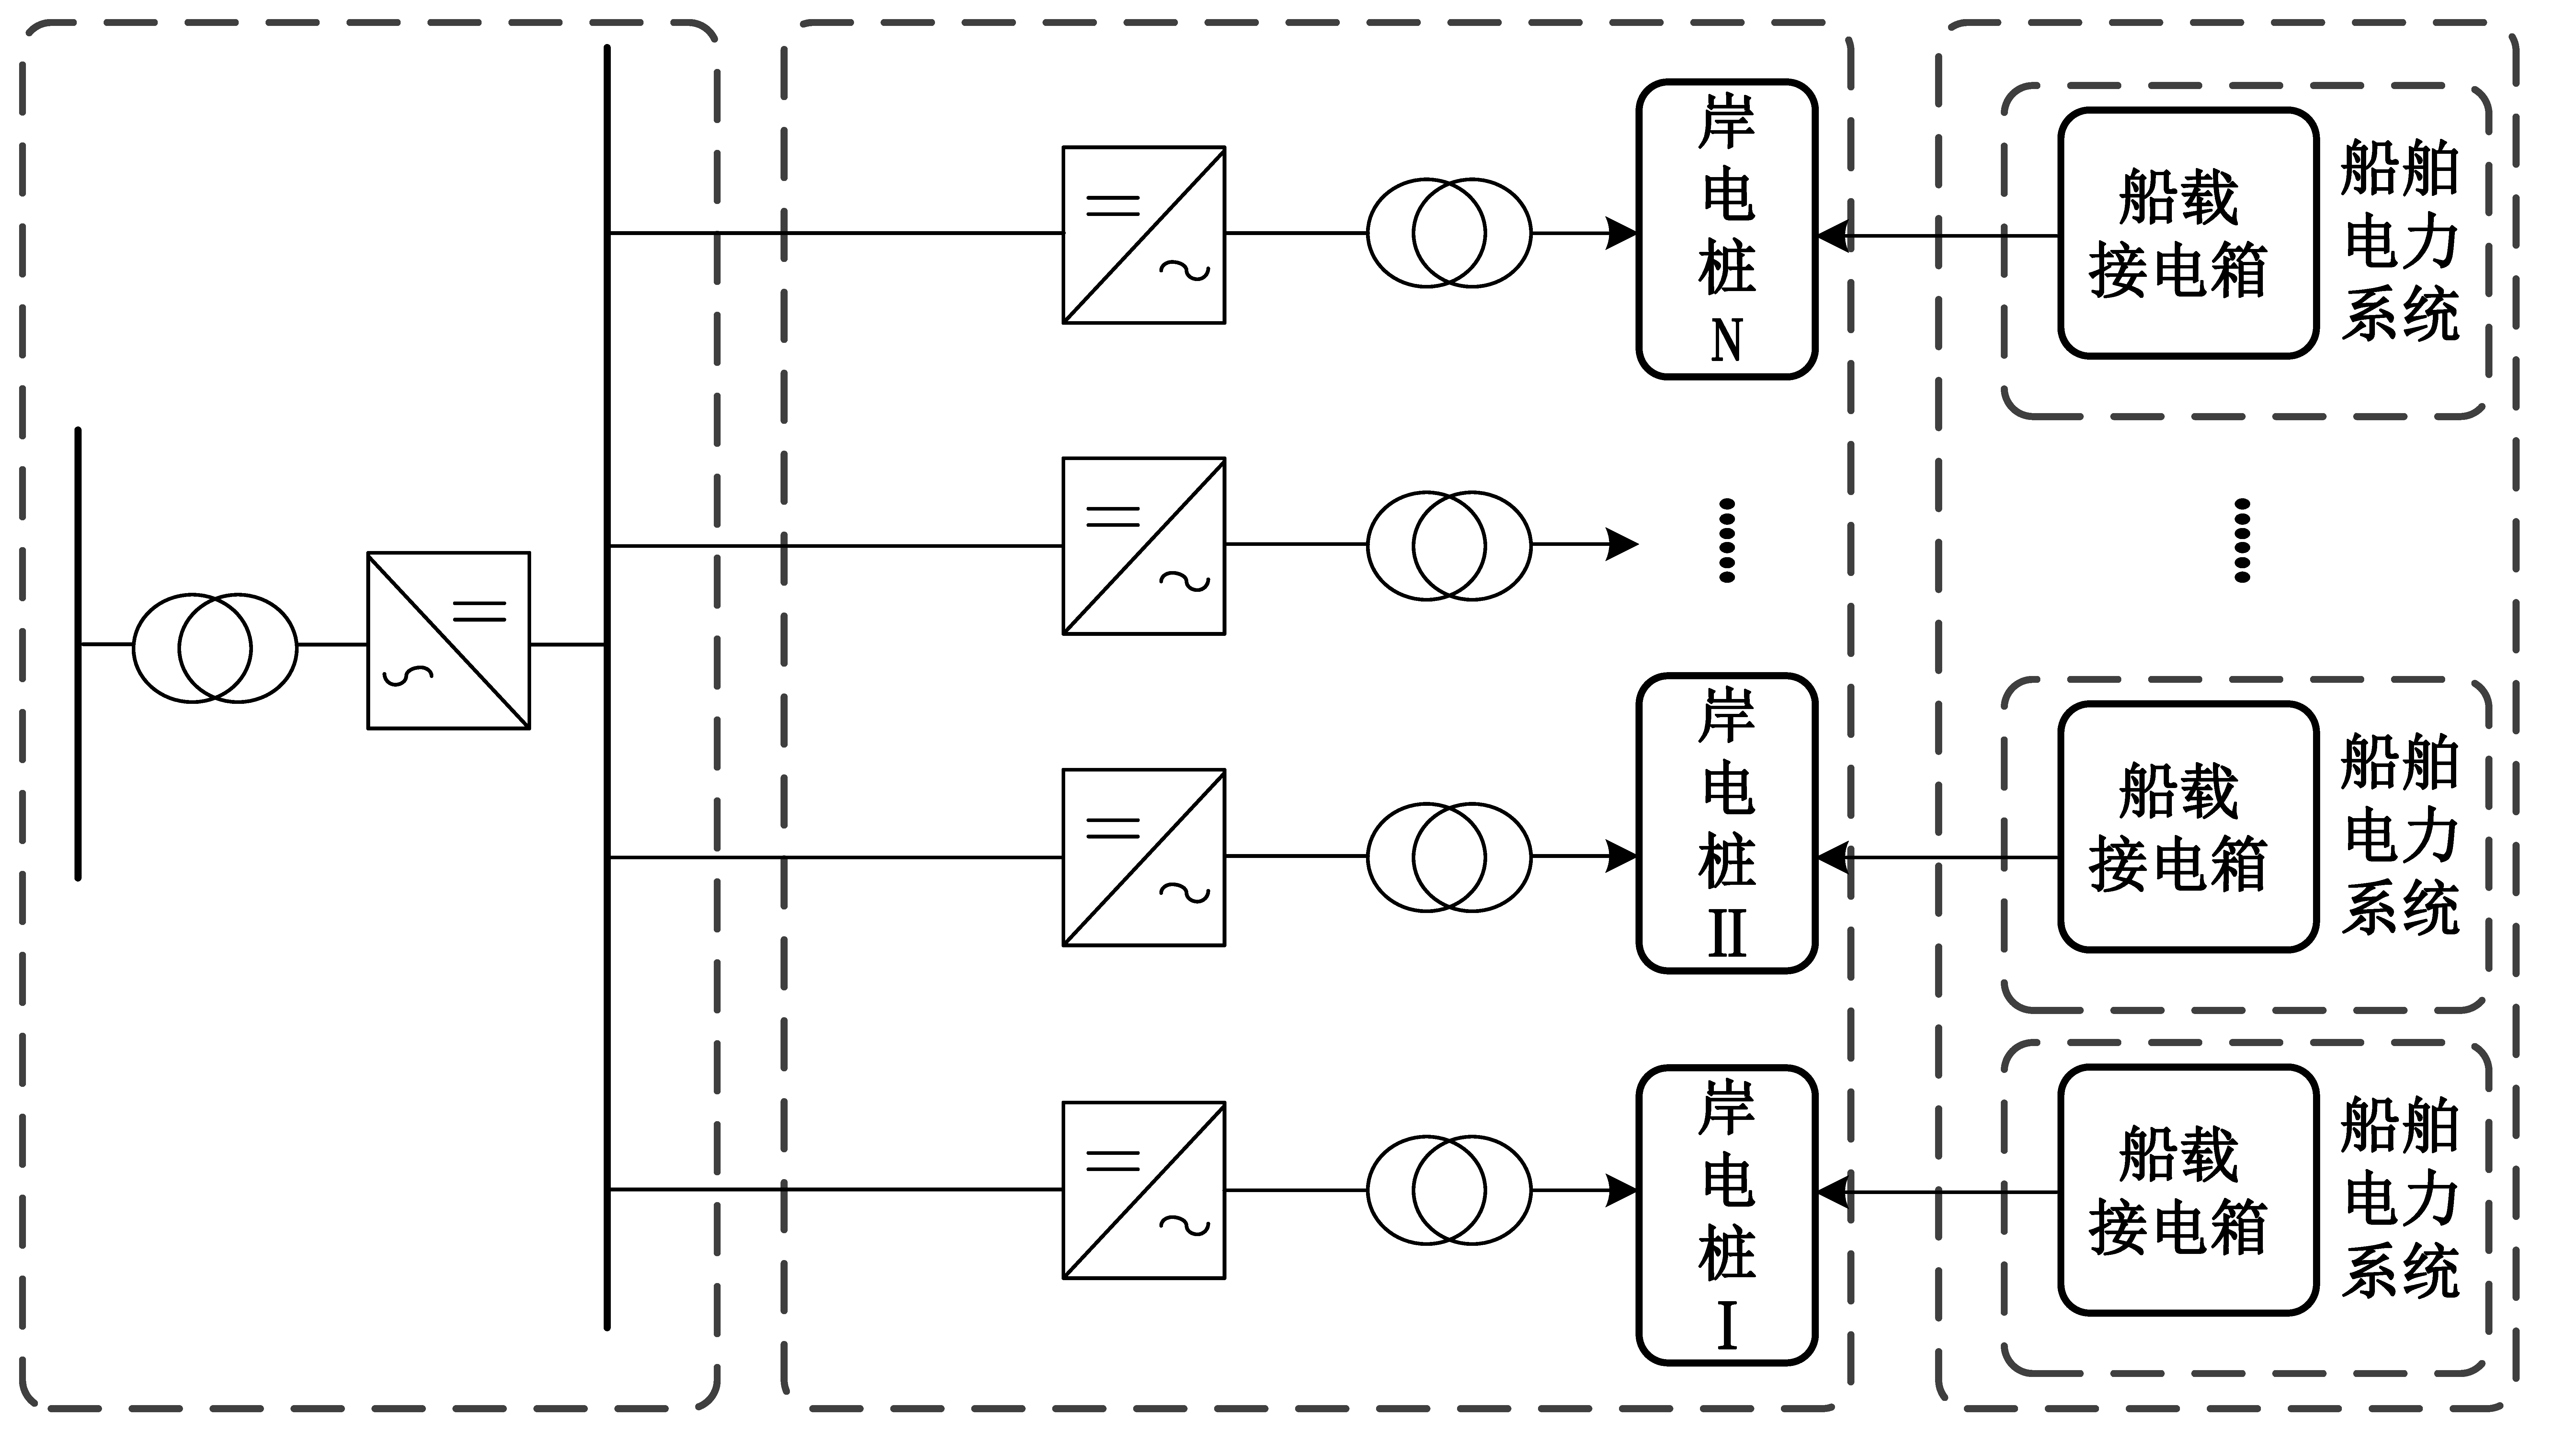
\includegraphics[width=0.9\textwidth]{chapter2/直流输电岸电电源.pdf}
	\caption{直流输电岸电结构}
	\label{fig:直流输电岸电结构}
\end{figure}

\section{船岸连接系统面临的问题}
\subsection{船舶岸电供电并网切换}
船岸电力的电网连接是在船的柴油发电机和岸上电源之间。并网需要满足四个条件:船舶发电机的相序、幅值、相位、频率
必须与岸电一致。保持相同的相序尤为重要。影响瞬时电压差的三个因素是频率差、相位差和电压差。船岸自动准同步并网
的四个条件如下:
(1)船舶电源的相序必须等于岸上电源的相序;
(2)船舶电源的电压幅值必须等于岸上电源的电压幅值;
(3)船舶电源的频率必须等于岸上电源的频率;
(4)船舶电源的相位必须等于岸上电源的相位。
这些条件在理想情况下得到满足。事实上,相位、频率和振幅不可能同时完全一致。但只要船电和岸电的相位、频率、幅度差
在一定值内,涌流就在系统可接受的范围内,所以可以进行船岸并网。

船舶岸电系统具备船电、岸电快速切换连接技术,通过船上同期装置,与岸电电源实现热并网,保证供电安全
可靠。船舶 岸电 系统接到岸电并网指令后,自动并车装置进行相序检测跟踪,在相序一致的情况 下,采集岸电电源及传
播辅机电源的电压、频率和相角差的信息,并计算判断是否满足以下并车条件:辅机与岸电的频率、相序及 电压幅值保持
一致,并且在并车的瞬间保证船舶辅机与岸电电源的输出电压相角同步。之后 完成并车并实现自动无缝负荷转移。根据船舶岸电
系统不同的供电连接方式,将岸电电源与船舶发电机的切换方式主要分为断电方式和无缝切换方式2种\cite{SP10}。
1)断电方式:当船舶靠港停泊时,需要首先使船舶上所有的用电设备关闭,并使船舶发电机停止工作,然后连接船舶岸电
系统,最后重新启动船舶的用电设备,实现船舶发电机与岸电电源之间的切换;当船舶离港时,按照相反的顺序操作。
2)同步并车方式:也被称为无缝切换方式,切换过程中不需要关闭 船上所有设备。同步并车方式不会影响船舶上用电设备
的正常运行,对船舶上的重要用电设备具有重大意义。无缝切换也是船舶岸电连接技术的发展趋势,对于岸电电源的推广
意义重大。船舶岸电自动并车技术需要保证船舶发电机与岸电电源的电压幅值和频率保持一致,并在并车的瞬间保证船舶发
电机与岸电电 源的输出电压相角同步。如果两路电源不同步就进行切换会造成严重的后果。如果在切换时刻一个电源电压波
形在波峰,另外一个位于波谷,切换过程中将会产生很大的冲击电流。虽然切换装置可能能承受该冲击电流,但严重时可能
会导致用电设备和高压静止频率变换器的自动保护装置动作。



\subsubsection{主动并网切换}
\subsubsection{被动并网切换}

\subsection{并网负载转移方式}
\subsection{逆功率处理方案}
\subsubsection{逆功率产生机理}
\subsubsection{逆功率的处理}
\subsubsection{不同控制方案简单对比}




\subsection{岸船连接段系统压降解决方案}

\subsubsection{隔离变压器的压降问题}
\subsubsection{输出电缆的压降问题}


\subsection{三相输出电压平衡控制技术}
\subsection{船岸等电位处理方案}



\section{本章小结}


